\documentclass[10pt, a4paper]{article}
\usepackage[top=80pt, bottom=50pt, left=72pt, right=55pt]{geometry}
\usepackage{enumerate}
\usepackage[fleqn]{amsmath}
\usepackage{graphicx}
\begin{document}
\title{PH-105 Assignment Sheet - 1}
\date{}
\author{Umang Mathur}
\maketitle
\begin{enumerate}
\item[10.] {\bf A light beam is propagating through a block of glass with index of refraction ($\eta$) 1.2. If the glass is moving at a constant velocity 0.8c in the same direction as beam what is the velocity of light in the block as observed by an observer in the laboratory? }\\

{\underline {\bf Solution}} :\\
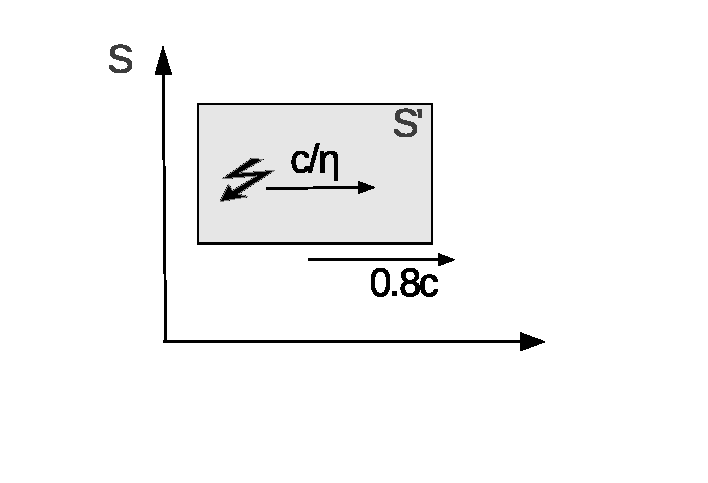
\includegraphics{fig2}\\
By the definition of refractive index, speed of light in S' = $c/\eta$

Now, using inverse velocity tramsformation and noting that $v = 0.8c$ and $u'_{x} = c/\eta$, we have:

\begin{align*}
	u_{x} &= \frac{u'_{x} + v}{1 + \frac{u'_{x}v}{c^{2}}}\\
	&= \frac{\frac{c}{1.2} + 0.8c}{1 + \frac{\frac{c}{1.2}0.8c}{c^{2}}}\\
	&= {\bf 0.98c}
\end{align*}

\end{enumerate}
\end{document} 
